% The \includeonly
% command can be used so you only need to work on one or two chapters at a
% time (instead of having to either latex the entire book each time or
% losing cross-references and page numbering)

\documentclass[12pt]{report}

\usepackage{suthesis-2e}
\usepackage{graphicx}
\usepackage{subcaption}
\usepackage{booktabs}
\usepackage{amsmath}
\usepackage{algorithm}
\usepackage{algpseudocode}

%% uncomment the following and create mythesis-macros.sty for all your
%% own macros.  This keeps this top level file looking fairly neat.
% \usepackage{mythesis-macros}
\DeclareMathOperator*{\argmax}{arg\,max}

    \title{Transcribing Real-Valued Sequences \\
           With Deep Neural Networks}
    \author{Awni Hannun}
    \principaladviser{Andrew Ng}
    \coprincipaladvisor{Dan Jurafsky}
    \firstreader{James Zou}
    \secondreader{Anshul Kundaje}

%\includeonly{first_pass}

\begin{document}

%% Preface

\beforepreface
\prefacesection{Abstract}

Speech recognition and arrhythmia detection from electrocardiograms are
examples of problems which can be formulated as transcribing real-valued
sequences. These problems have traditionally been solved with frameworks like
the Hidden Markov Model. To generalize well, these models rely on carefully
hand engineered building blocks. More general, end-to-end neural networks
capable of learning from much larger datasets can achieve lower error rates.
However, getting these models to work well in practice has other challenges.

In this work, we present end-to-end models for transcribing real-valued
sequences and discuss several applications of these models. The first is
detecting abnormal heart activity in electrocardiograms. The second is large
vocabulary continuous speech recognition. Finally, we investigate the tasks of
keyword spotting and voice activity detection. In all cases we show how to
scale high capacity models to unprecedentedly large datasets. With these
techniques we can achieve performance comparable to that of human experts for
both arrhythmia detection and speech recognition and state-of-the-art error
rates in speech recognition for multiple languages.


% dedication
\newpage
\begin{center}
    To person.
\end{center}

% the last preface section (e.g., acknowledgement.tex)
% should look like

\prefacesection{Acknowledgements}

So many people have contributed to the completion of my PhD. It's safe to say
that this thesis would not have been possible were it not for the great
collaborators I've had the good fortune of working with as well as my family
and friends who supported me every day.

First, I'd like to thank my family. My entire family and especially my parents,
Lina and Yusuf, have always unconditionally supported me in my career choices
and inspired me in my work. I am also very grateful to my wife Kathy who first
inspired me to come back to school while I was working at Google and has been
with me every day since.

I would also like to thank my advisor Andrew Ng and co-advisor Dan Jurafsky.
Dan's constant positive encouragement, enthusiasm and mentorship over the past
six years have made the research not only possible but enjoyable.

I owe so much of my success in this work now and in the future to Andrew
directly or indirectly given that he has trained so many of my close mentors
and collaborators. Andrew has been a guide to me on all possible fronts
including technically and strategically in research and in all of the softer
skills which are critical to doing impactful work.

My first forray into machine learning research was during my time at Google,
where I had the pleasure to be mentored by Quoc Le. Quoc introduced me to the
just burgeoning field of deep learning and Andrew Ng's lab at Stanford. For
this I am very grateful. I am also grateful to Andrew Maas for taking me under
his wing during my first two years at Stanford. Andrew M. taught me a lot about
machine learning and speech recognition. During that period I also had the good
fortune of getting to know and work with many people in Andrew Ng's lab
including Chris Lengerich, Peng Qi, Richard Socher, Brody Huval, Ziang Xie,
Anshul Samar, Tao Wang, Sameep Tandon and Adam Coates.

I then spent close to two years as a Research Scientist at Baidu's newly formed
Silicon Valley AI lab under the leadership of Adam Coates and Andrew Ng. This
was a life changing experience for me and I couldn't be more grateful to have
had Adam Coates as a close mentor and friend during that time and since.

I'm grateful to the entire Deep Speech team. As I now know, it's a rare thing
indeed to work with such a highly productive and enjoyable group. The Deep
Speech collaborators include Carl Case, Jared Casper, Bryan Catanzaro, Greg
Diamos, Erich Elsen, Ryan Prenger, Sanjeev Satheesh, Shubho Sengupta, Adam
Coates and Andrew Ng. Thank you all for being a part of such an exciting time
and teaching me so much then and since. I would also like to thank the Deep
Speech 2 team at Baidu and all of my collaborators there. There are too many to
list invidually, but a few others that I worked closely with during that time
include Dario Amodei, Jesse Engel, Eric Battenberg, Sherjil Ozair, Chong Wang,
Tony Han, Jim Fan and Zhenyao Zhu.

I would also like to thank Chris Lengerich for being my collaborator in the
start-up world and on many research projects over the years.

After returning to Stanford from Baidu Research, I ventured into machine
learning applications for healthcare. During this time I had the good fortune
to work with Pranav Rajpurkar, Geoffrey Tison, Mintu Turakhia and several
employees at iRhythm Technologies including Masoumeh Haghpanahi, Codie Bourn
and Justin Cambra. I am also grateful to my office mates Anand Avati and Ziang
Xie as well as many other lab members including Sudnya Diamos, Dillon Laird,
Jeremy Irvin, James Liu and Will Hang.

I'd like to thank Swati Dube for kicking-off and organizing many fruitful
parternships between our lab at Stanford and other organizations. Also thanks
to the lab administrative staff and PhD student services staff for all their
help over the years.

Thanks to my reading committee James Zou, Anshul Kundaje, Dan and Andrew for
their feedback and advice as well as my thesis defense chair Nigam Shah.

Thanks to everyone who made this work possible through collaboration,
mentorship, support, encouragement and of course friendship and entertainment.

\afterpreface



%% Chapters
\section{Introduction}
\label{sec:scaling_asr:introduction}

Decades worth of hand-engineered domain knowledge has gone into current
state-of-the-art automatic speech recognition (ASR) pipelines.  A simple but
powerful alternative solution is to train such ASR models end-to-end, using
deep learning to replace most modules with a single
model~\cite{hannun2014deepspeech}. We present the second generation of our
speech system that exemplifies the major advantages of end-to-end learning. The
{Deep Speech 2} ASR pipeline approaches or exceeds the accuracy of Amazon
Mechanical Turk human workers on several benchmarks, works in multiple
languages with little modification, and is deployable in a production setting.
It thus represents a significant step towards a single ASR system that
addresses the entire range of speech recognition contexts handled by humans.
Since our system is built on end-to-end deep learning, we can employ a spectrum
of deep learning techniques: capturing large training sets, training larger
models with high performance computing, and methodically exploring the space of
neural network architectures. We show that through these techniques we are able
to reduce error rates of our previous end-to-end
system~\cite{hannun2014deepspeech} in English by up to 43\%, and can also
recognize Mandarin speech with high accuracy.

One of the challenges of speech recognition is the wide range of variability in
speech and acoustics. As a result, modern ASR pipelines are made up of numerous
components including complex feature extraction, acoustic models, language and
pronunciation models, speaker adaptation, etc. Building and tuning these
individual components makes developing a new speech recognizer very hard,
especially for a new language.  Indeed, many parts do not generalize well
across environments or languages and it is often necessary to support multiple
application-specific systems in order to provide acceptable accuracy. This
state of affairs is different from human speech recognition: people have the
innate ability to learn any language during childhood, using general skills to
learn language. After learning to read and write, most humans can transcribe
speech with robustness to variation in environment, speaker accent and noise,
without additional training for the transcription task.  To meet the
expectations of speech recognition users, we believe that a single engine must
learn to be similarly competent; able to handle most applications with only
minor modifications and able to learn new languages from scratch without
dramatic changes.  Our end-to-end system puts this goal within reach, allowing
us to approach or exceed the performance of human workers on several tests in
two very different languages: Mandarin and English.

Since {Deep Speech 2} (DS2) is an end-to-end deep learning system, we can
achieve performance gains by focusing on three crucial components:  the model
architecture, large labeled training datasets, and computational scale. This
approach has also yielded great advances in other application areas such as
computer vision and natural language.  This paper details our contribution to
these three areas for speech recognition, including an extensive investigation
of model architectures and the effect of data and model size on recognition
performance.  In particular, we describe numerous experiments with neural
networks trained with the Connectionist Temporal Classification (CTC) loss
function~\cite{graves2006} to predict speech transcriptions from audio.  We
consider networks composed of many layers of recurrent connections,
convolutional filters, and nonlinearities, as well as the impact of a specific
instance of Batch Normalization~\cite{ioffe2015batch} (BatchNorm) applied to
RNNs.  We not only find networks that produce much better predictions than
those in previous work~\cite{hannun2014deepspeech}, but also find instances of
recurrent models that can be deployed in a production setting with no
significant loss in accuracy.

Beyond the search for better model architecture, deep learning systems benefit
greatly from large quantities of training data.  We detail our data capturing
pipeline that has enabled us to create larger datasets than what is typically
used to train speech recognition systems.  Our English speech system is trained
on 11,940 hours of speech, while the Mandarin system is trained on 9,400 hours.
We use data synthesis to further augment the data during training.

Training on large quantities of data usually requires the use of larger models.
Indeed, our models have many more parameters than those used in our previous
system. Training a single model at these scales requires tens of
exaFLOPs\footnote{1 exaFLOP = $10^{18}$ FLoating-point OPerations.} that would
require 3-6 weeks to execute on a single GPU. This makes model exploration a
very time consuming exercise, so we have built a highly optimized training
system that uses 8 or 16 GPUs to train one model. In contrast to previous
large-scale training approaches that use parameter servers and asynchronous
updates~\cite{dean2012, chilimbi2014}, we use synchronous SGD, which is easier
to debug while testing new ideas, and also converges faster for the same degree
of data parallelism. To make the entire system efficient, we describe
optimizations for a single GPU as well as improvements to scalability for
multiple GPUs. We employ optimization techniques typically found in High
Performance Computing to improve scalability. These optimizations include a
fast implementation of the CTC loss function on the GPU, and a custom memory
allocator. We also use carefully integrated compute nodes and a custom
implementation of all-reduce to accelerate inter-GPU communication. Overall the
system sustains approximately 50 teraFLOP/second when training on 16 GPUs. This
amounts to 3 teraFLOP/second per GPU which is about 50\% of peak theoretical
performance. This scalability and efficiency cuts training times down to 3 to 5
days, allowing us to iterate more quickly on our models and datasets.

We benchmark our system on several publicly available test sets and compare the
results to our previous end-to-end system~\cite{hannun2014deepspeech}.  Our
goal is to eventually reach human-level performance not only on specific
benchmarks, where it is possible to improve through dataset-specific tuning,
but on a range of benchmarks that reflects a diverse set of scenarios. To that
end, we have also measured the performance of human workers on each benchmark
for comparison.  We find that our system outperforms humans in some
commonly-studied benchmarks and has significantly closed the gap in much harder
cases.  In addition to public benchmarks, we show the performance of our
Mandarin system on internal datasets that reflect real-world product scenarios.

Deep learning systems can be challenging to deploy at scale.  Large neural
networks are computationally expensive to evaluate for each user utterance, and
some network architectures are more easily deployed than others. Through model
exploration, we find high-accuracy, deployable network architectures, which we
detail here. We also employ a batching scheme suitable for GPU hardware called
Batch Dispatch that leads to an efficient, real-time implementation of our
Mandarin engine on production servers.  Our implementation achieves a 98th
percentile compute latency of 67 milliseconds, while the server is loaded with
10 simultaneous audio streams.

\chapter{Application to Arrhythmia Detection}

% TODOs
% Check section labelling
% Update text to reflext Lancet submission

\section{Introduction}
\label{sec:arrhythmias:intro}

We develop a model which can diagnose irregular heart rhythms, also known as
arrhythmias, from single-lead ECG signals better than a cardiologist. Key to
exceeding expert performance is a deep convolutional network which can map a
sequence of ECG samples to a sequence of arrhythmia annotations along with a
novel dataset two orders of magnitude larger than previous datasets of its
kind.

Many heart diseases, including Myocardial Infarction, AV Block, Ventricular
Tachycardia and Atrial Fibrillation can all be diagnosed from ECG signals with
an estimated 300 million ECGs recorded annually~\cite{heden1996detection}. We
investigate the task of arrhythmia detection from the ECG record. This is known
to be a challenging task for computers but can usually be determined by an
expert from a single, well-placed lead.

Arrhythmia detection from ECG recordings is usually performed by expert
technicians and cardiologists given the high error rates of computerized
interpretation.  One study found that of all the computer predictions for
non-sinus rhythms, only about 50\% were correct~\cite{shah2007errors}; in
another study, only 1 out of every 7 presentations of second degree AV block
were correctly recognized by the algorithm~\cite{guglin2006common}. To
automatically detect heart arrhythmias in an ECG, an algorithm must implicitly
recognize the distinct wave types and discern the complex relationships between
them over time. This is difficult due to the variability in wave morphology
between patients as well as the presence of noise.

We train a 34-layer convolutional neural network (CNN) to detect arrhythmias in
arbitrary length ECG time-series. Figure~\ref{fig:record} shows an example of
an input to the model. In addition to classifying noise and the sinus rhythm,
the network learns to classify and segment twelve arrhythmia types present in
the time-series. The model is trained end-to-end on a single-lead ECG signal
sampled at 200Hz and a sequence of annotations for every second of the ECG as
supervision. To make the optimization of such a deep model tractable, we use
residual connections and batch-normalization~\cite{he2016deep, ioffe2015batch}.
The depth increases both the non-linearity of the computation as well as the
size of the context window for each classification decision.

We construct a dataset 500 times larger than other datasets of its
kind~\cite{moody2001impact, goldberger2000physiobank}. One of the most popular
previous datasets, the MIT-BIH corpus contains ECG recordings from 47 unique
patients. In contrast, we collect and annotate a dataset of about 30,000 unique
patients from a pool of nearly 300,000 patients who have used the Zio Patch
monitor\footnote[1]{iRhythm Technologies, San Francisco,
California}~\cite{turakhia2013diagnostic}. We intentionally select patients
exhibiting abnormal rhythms in order to make the class balance of the dataset
more even and thus the likelihood of observing unusual heart-activity high.

We test our model against board-certified cardiologists. A committee of three
cardiologists serve as gold-standard annotators for the 336 examples in the
test set. Our model exceeds the individual expert performance on both recall
(sensitivity), and precision (positive predictive value) on this test set.

\section{Related Work}
\label{sec:arrhythmia:related}

Automatic high-accuracy methods for R-peak extraction have existed at least
since the mid 1980's \cite{pan1985real}. Current algorithms for R-peak
extraction tend to use wavelet transformations to compute features from the raw
ECG followed by finely-tuned threshold based classifiers \cite{li1995detection,
martinez2004wavelet}. Because accurate estimates of heart rate and heart rate
variability can be extracted from R-peak features, feature-engineered
algorithms are often used for coarse-grained heart rhythm classification,
including detecting tachycardias (fast heart rate), bradycardias (slow heart
rate), and irregular rhythms. However, such features alone are not sufficient
to distinguish between most heart arrhythmias since features based on the
atrial activity of the heart as well as other features pertaining to the QRS
morphology are needed.

Much work has been done to automate the extraction of other features from the
ECG. For example, beat classification is a common sub-problem of
heart-arrhythmia classification. Drawing inspiration from automatic speech
recognition, Hidden Markov models with Gaussian observation probability
distributions have been applied to the task of beat detection
\cite{coast1990approach}. Artificial neural networks have also been used for
the task of beat detection \cite{melo2000arrhythmia}. While these models have
achieved high-accuracy for some beat types, they are not yet sufficient for
high-accuracy heart arrhythmia classification and segmentation. For example,
\cite{artis1991detection} train a neural network to distinguish between Atrial
Fibrillation and Sinus Rhythm on the MIT-BIH dataset. While the network can
distinguish between these two classes with high-accuracy, it does not
generalize to noisier single-lead recordings or classify among the full range
of $15$ rhythms available in MIT-BIH. This is in part due to insufficient
training data, and because the model also discards critical information in the
feature extraction stage.

The most common dataset used to design and evaluate ECG algorithms is the
MIT-BIH arrhythmia database \cite{moody2001impact} which consists of 48
half-hour strips of ECG data. Other commonly used datasets include the MIT-BIH
Atrial Fibrillation dataset \cite{moody1983new} and the QT dataset
\cite{laguna1997database}. While useful benchmarks for R-peak extraction and
beat-level annotations, these datasets are too small for fine-grained
arrhythmia classification. The number of unique patients is in the single digit
hundreds or fewer for these benchmarks. A recently released dataset captured
from the AliveCor ECG monitor contains about 7000 records \cite{clifford2017}.
These records only have annotations for Atrial Fibrillation; all other
arrhythmias are grouped into a single bucket. The dataset we develop contains
29,163 unique patients and $14$ classes with hundreds of unique examples for
the rarest arrhythmias.

Machine learning models based on deep neural networks have consistently been
able to approach and often exceed human agreement rates when large annotated
datasets are available \cite{amodei2016deep, xiong2016achieving,he2015delving}.
These approaches have also proven to be effective in healthcare applications,
particularly in medical imaging where pretrained ImageNet models can be applied
\cite{esteva2017dermatologist, gulshan2016development}. We draw on work in
automatic speech recognition for processing time-series with deep convolutional
neural networks and recurrent neural networks \cite{hannun2014deepspeech,
sainath2013deep}, and techniques in deep learning to make the optimization of
these models tractable \cite{he2016deep, he2016identity, ioffe2015batch}.

\section{Model}
\label{sec:arrhythmias:model}

\subsection{Problem Formulation}

The ECG arrhythmia detection task is a sequence-to-sequence task which takes as
input an ECG signal $X=[x_1,.. x_T]$, and outputs a sequence of labels $Y=[y_1,
... y_U]$, such that each $y_u$ can take on one of 12 different rhythm
classes. Each output label corresponds to a segment of the input. Together the
output labels cover the full sequence.

For a single example in the training set, we optimize the cross-entropy
objective function
\[
 \mathcal{L}(X, Y) = \frac{1}{U} \sum_{u=1}^U \log p(y_u \mid X)
\]
where $p(\cdot)$ is the probability that the network assigns to the $u$-th
output taking on the value $y_u$.

\subsection{Model Architecture and Training}

We use a convolutional neural network for the sequence-to-sequence learning
task. The high-level architecture of the network is shown in
Figure~\ref{fig:arrhythmias:net}. The network takes as input a time-series of
raw ECG signal, and outputs a sequence of label predictions. The 30 second long
ECG signal is sampled at 200Hz, and the model outputs a new prediction once
every 256 samples. After careful architectur search, arrive at a model which is
33 layers of convolution followed by a fully connected layer and a softmax. 

\begin{figure}
\centering
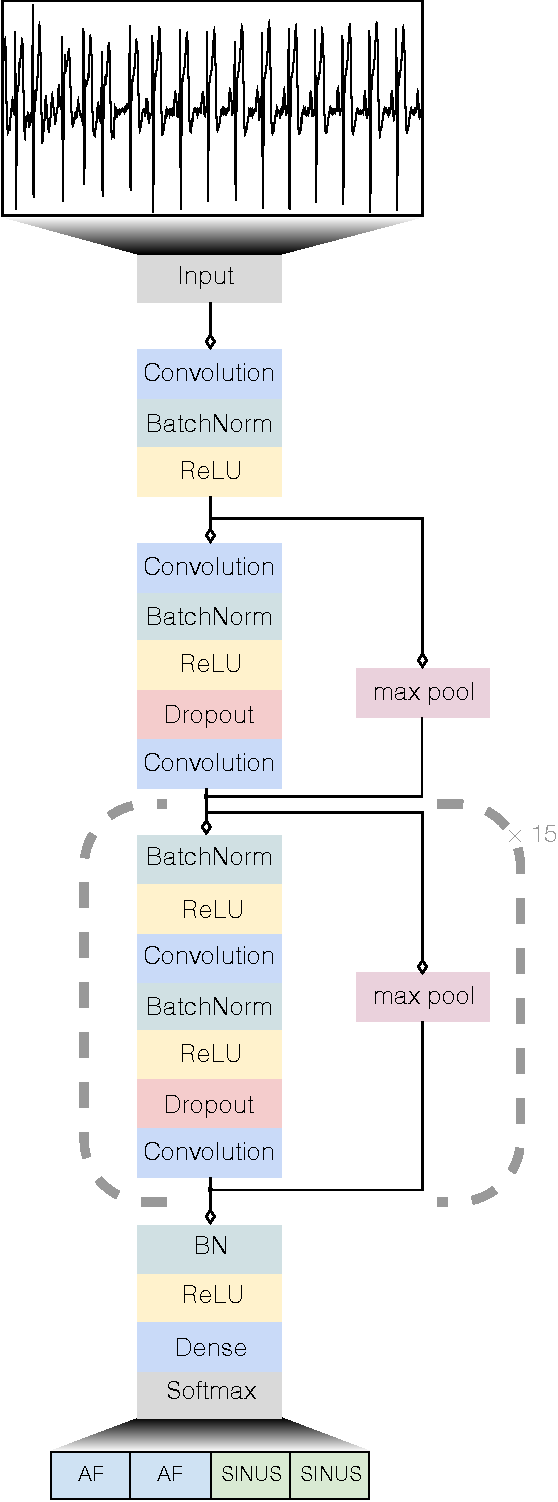
\includegraphics[width=0.4\textwidth]{arrhythmias/figures/ecg_network_full.pdf}
\caption{The architecture of the deep neural network consists of 33
         convolutional layers followed by a fully-connected layer and
         a softmax layer.}
\label{fig:arrhythmias:net}
\end{figure}

In order to make the optimization of such a network tractable, we employ
shortcut connections in a similar manner to those found in the Residual Network
architecture~\cite{he2016identity}. The shortcut connections between
neural-network layers optimize training by allowing information to propagate
well in very deep neural networks. Before the input is fed into the network, it
is normalized using a robust normalization strategy. The network consists of 16
residual blocks with 2 convolutional layers per block. The convolutional layers
all have a filter length of 16 and have 64$k$ filters, where $k$ starts out as
1 and is incremented every 4-th residual block. Every alternate residual block
subsamples its inputs by a factor of 2, thus the original input is ultimately
subsampled by a factor of $2^8$. When a residual block subsamples the input,
the corresponding shortcut connections also subsample their input using a Max
Pooling operation with the same subsample factor. 

Before each convolutional layer we apply Batch
Normalization~\cite{ioffe2015batch} and a rectified linear activation, adopting
the pre-activation block design~\cite{he2016deep}. The first and last layers of
the network are special-cased due to this pre-activation block structure. We
also apply Dropout~\cite{srivastava2014dropout} between the convolutional
layers and after the non-linearity. The final fully connected layer and softmax
activation produce a distribution over the 12 output classes for each
time-step.

We train the networks from scratch, initializing the weights of the
convolutional layers as in~\cite{he2015delving}. We use the
Adam~\cite{kingma2014adam} optimizer with the default parameters and reduce the
learning rate by a factor of 10 when the validation loss stops improving. We
save the best model as evaluated on the validation set during the optimization
process.

\section{Datasets}
\label{arrhythmia:sec:data}

\subsection*{Training}
We collect and annotate a dataset of 64,121 ECG records from 29,163 patients.
The ECG data is sampled at a frequency of 200 Hz and is collected from a
single-lead, noninvasive and  continuous monitoring device called the Zio Patch
which has a wear period up to 14 days \cite{turakhia2013diagnostic}. Each ECG
record in the training set is 30 seconds long and can contain more than one
rhythm type. Each record is annotated by a clinical ECG expert: the expert
highlights segments of the signal and marks it as corresponding to one of the
14 rhythm classes.

The 30 second records were annotated using a web-based ECG annotation tool
designed for this work. Label annotations were done by a group of Certified
Cardiographic Technicians who have completed extensive training in arrhythmia
detection and a cardiographic certification examination by Cardiovascular
Credentialing International. The technicians were guided through the interface
before they could annotate records. All rhythms present in a strip were labeled
from their corresponding onset to offset, resulting in full segmentation of the
input ECG data. To improve labeling consistency among different annotators,
specific rules were devised regarding each rhythm transition.

We split the dataset into a training and validation set. The training set
contains 90\% of the data. We split the dataset so that there is no patient
overlap between the training and validation sets (as well as the test set
described below).

\subsection*{Testing}

We collect a test set of 336 records from 328 unique patients. For the test
set, ground truth annotations for each record were obtained by a committee of
three board-certified cardiologists; there are three committees responsible for
different splits of the test set. The cardiologists discussed each individual
record as a group and came to a consensus labeling. For each record in the test
set we also collect 6 individual annotations from cardiologists not
participating in the group. This is used to assess performance of the model
compared to an individual cardiologist.

\subsection*{Rhythm Classes}
We identify 12 heart arrhythmias, sinus rhythm and noise for a total of 14
output classes. The arrhythmias are characterized by a variety of features.
Table~\ref{tab:rhythms} in the Appendix shows an example of each rhythm type we
classify. The noise label is assigned when the device is disconnected from the
skin or when the baseline noise in the ECG makes identification of the
underlying rhythm impossible.

The morphology of the ECG during a single heart-beat as well as the pattern of
the activity of the heart over time determine the underlying rhythm. In some
cases the distinction between the rhythms can be subtle yet critical for
treatment. For example two forms of second degree AV Block, Mobitz I
(Wenckebach) and Mobitz II (here referred to as AVB\_TYPE2) can be difficult to
distinguish. Wenckebach is considered benign and Mobitz II is considered
pathological, requiring immediate attention \cite{dubin1996rapid}. 

Table~\ref{tab:rhythms} in the Appendix also shows the number of unique
patients in the training (including validation) set and test set for each
rhythm type.

\section{Experimental Results}

\subsection*{Evaluation Metrics}
We use two metrics to measure model accuracy, using the cardiologist committee
annotations as the ground truth.

\textbf{Sequence Level Accuracy (F1):} We measure the average overlap between
the prediction and the ground truth sequence labels. For every record, a model
is required to make a prediction approximately once per second (every 256
samples). These predictions are compared against the ground truth annotation.

\textbf{Set Level Accuracy (F1):} Instead of treating the labels for a record
as a sequence, we consider the set of unique arrhythmias present in each 30
second record as the ground truth annotation. Set Level Accuracy, unlike
Sequence Level Accuracy, does not penalize for time-misalignment within a
record. We report the F1 score between the unique class labels from the ground
truth and those from the model prediction.

In both the Sequence and the Set case, we compute the metrics for each class
separately. We then compute aggregate results for AUC and F1 as the
class-frequency weighted mean.

\subsection*{Model and Cardiologist Performance}

We assess the cardiologist performance on the test set. Recall that each of the
records in the test set has a ground truth label from a committee of three
cardiologists as well as individual labels from a disjoint set of 6 other
cardiologists. To assess cardiologist performance for each class, we take the
average of all the individual cardiologist scores using the group label as the
ground truth annotation.

\begin{table}
\centering
\begin{small}
\begin{tabular}{r l l}
\toprule
                               & Sequence AUC & Set AUC \\
\midrule
Atrial Fibrillation \& Flutter & 0.975 & 0.959 \\
Atrio-ventricular Block        & 0.989 & 0.981 \\
Bigeminy                       & 0.998 & 0.997 \\
Ectopic Atrial Rhythm          & 0.908 & 0.935 \\
Idioventricular Rhythm         & 0.995 & 0.986 \\
Junctional Rhythm              & 0.985 & 0.980 \\
Noise                          & 0.985 & 0.958 \\
Sinus Rhythm                   & 0.976 & 0.981 \\
Supraventricular Tachycardia   & 0.972 & 0.940 \\
Trigeminy                      & 0.999 & 0.997 \\
Ventricular Tachycardia        & 0.995 & 0.981 \\
Wenckebach                     & 0.982 & 0.981 \\
\midrule
   Average                     & 0.979               & 0.974 \\
\bottomrule
\end{tabular}
\end{small}
\caption{The model AUC scores for each rhythm class and in aggregate.}
\label{tab:arrhythmias:model_auc}
\end{table}

Table~\ref{tab:arrhythmias:model_auc} gives the per class and aggregate AUC
scores. Our model achieves an AUC of greater than 0.90 for each of the 12
rhythm diagnoses, with an average AUC of 0.97. We also compute the sensitivity
at a specifity of 0.9 and vice versa in~\ref{tab:arrhythmias:sens_spec}.

\begin{table}
\centering
\begin{small}
\begin{tabular}{r l l}
\toprule
             & Sensitivity       & Specificity  \\
\midrule
Atrial Fibrillation \& Flutter & 0.923 & 0.914 \\
Atrio-ventricular Block        & 0.991 & 0.964 \\
Bigeminy                       & 1.000 & 0.997 \\
Ectopic Atrial Rhythm          & 0.754 & 0.665 \\
Idioventricular Rhythm         & 0.990 & 0.990 \\
Junctional Rhythm              & 0.982 & 0.959 \\
Noise                          & 0.965 & 0.968 \\
Sinus Rhythm                   & 0.934 & 0.946 \\
Supraventricular Tachycardia   & 0.958 & 0.925 \\
Trigeminy                      & 1.000 & 0.999 \\
Ventricular Tachycardia        & 1.000 & 0.981 \\
Wenckebach                     & 0.977 & 0.956 \\
\bottomrule
\end{tabular}
\end{small}
\caption{The maximum model sensitivity with specificity greater than 0.9 and
         vice versa.}
\label{tab:arrhythmias:sens_spec}
\end{table}

\begin{table}
\centering
\begin{small}
\begin{tabular}{r c c c c}
\toprule
    & \multicolumn{2}{c}{Sequence F1} & \multicolumn{2}{c}{Set F1} \\
\cmidrule{2-5}
 & Model & Cardiol. & Model & Cardiol. \\
\midrule
Atrial Fibrillation \& Flutter & 0.802 & 0.679 & 0.817 & 0.687 \\
Atrio-ventricular Block        & 0.850 & 0.769 & 0.830 & 0.756 \\
Bigeminy                       & 0.896 & 0.837 & 0.870 & 0.849 \\
Ectopic Atrial Rhythm          & 0.537 & 0.476 & 0.545 & 0.529 \\
Idioventricular Rhythm         & 0.751 & 0.632 & 0.818 & 0.720 \\
Junctional Rhythm              & 0.640 & 0.684 & 0.778 & 0.674 \\
Noise                          & 0.852 & 0.768 & 0.704 & 0.689 \\
Sinus Rhythm                   & 0.886 & 0.847 & 0.934 & 0.907 \\
Supraventricular Tachycardia   & 0.458 & 0.449 & 0.630 & 0.556 \\
Trigeminy                      & 0.909 & 0.843 & 0.870 & 0.816 \\
Ventricular Tachycardia        & 0.520 & 0.566 & 0.653 & 0.769 \\
Wenckebach                     & 0.714 & 0.593 & 0.806 & 0.736 \\
\midrule
Average	                       & 0.808 & 0.750 & 0.809 & 0.778 \\
\bottomrule
\end{tabular}
\end{small}
\caption{The F1 score for the sequence and set-level metrics comparing the
         model and the average of six individual cardiologist to the committee
         consensus ground truth.}
\label{tab:arrhythmias:model_cardiologist_f1}
\end{table}

Table~\ref{tab:arrhythmias:model_cardiologist_f1} shows the breakdown of both
cardiologist and model sequence and set F1 across the different rhythm classes.
The model outperforms the average cardiologist performance on most rhythms,
noticeably outperforming the cardiologists in the AV Block set of arrhythmias
which includes Mobitz I (Wenckebach), Mobitz II and complete heart block (both
categorized as Atrio-ventricular Block). This is especially useful given the
severity of second and third degree heart block and the importance of
distinguishing these two from Wenckebach which is usually considered benign.
The model also outperforms the cardiologist average accross all rhythm classes
for both the sequence and set F1 score.

\begin{figure}
\centering
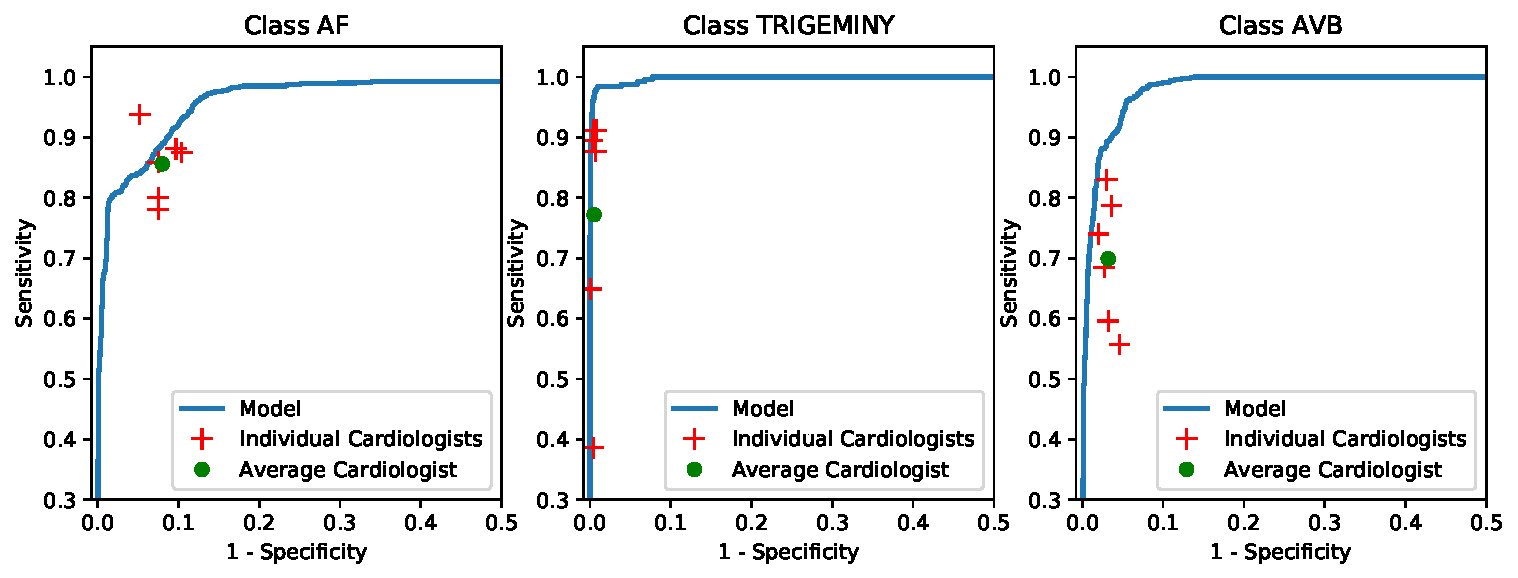
\includegraphics[width=1.0\textwidth]{arrhythmias/figures/roc_curve.pdf}
\caption{Receiver operating characteristic curves at the sequence level for
    atrial fibrillation and flutter (AF), trigeminy and atrioventricular block
    (AVB).}
\label{fig:arrhythmias:roc_curve}
\end{figure}

Figures~\ref{fig:arrhythmias:roc_curve} and
\ref{fig:arrhythmias:prec_recall_curve} show the models performance at various
operating thresholds on an ROC and precision-recall curve respectively. We show
here three arrhythmias taken from one-third of the test set. We also compute
and plot the operating point for the six individual cardiologists who annotated
that third of the test set. The model outperforms almost all of the individual
cardiologists. We see the same behaviour for the other rhythm classes not shown
here.

\begin{figure}
\centering
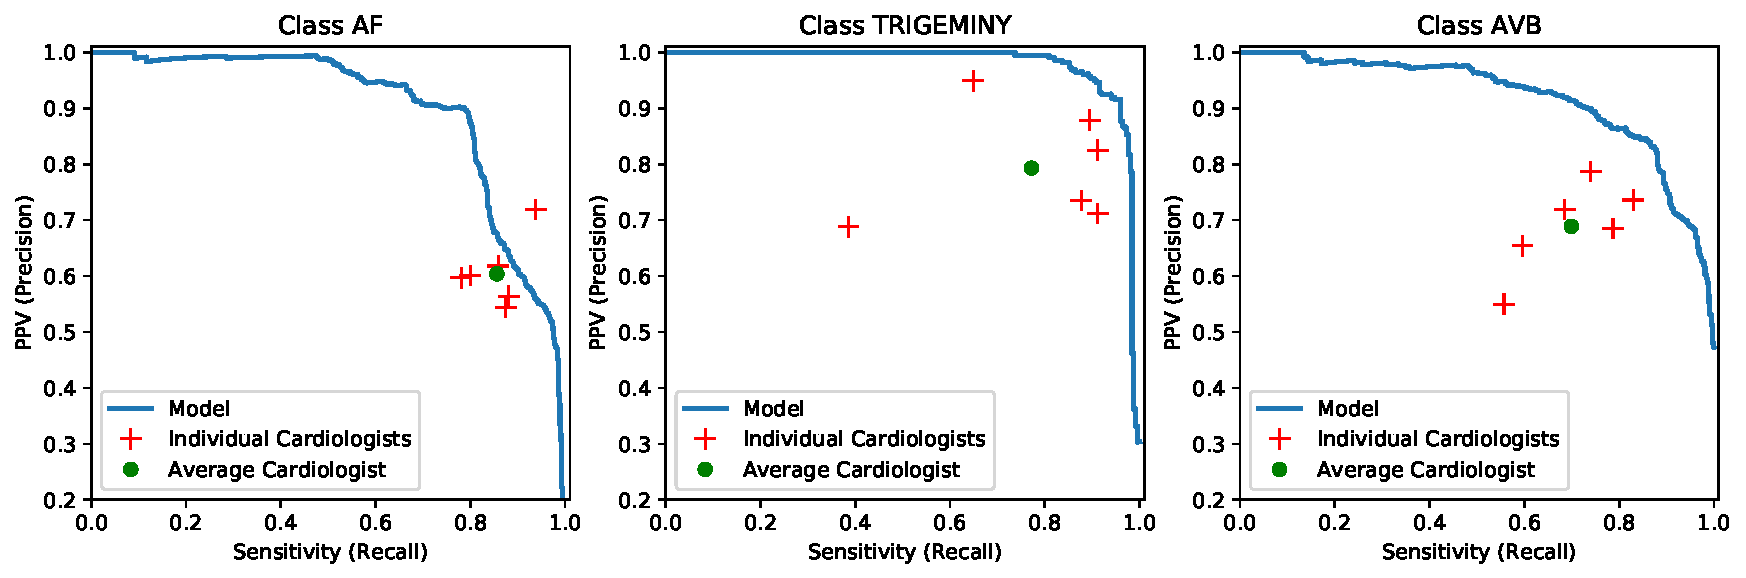
\includegraphics[width=1.0\textwidth]{arrhythmias/figures/prec_recall_curve.pdf}
    \caption{Precision-recall curves at the sequence level for atrial
    fibrillation and flutter (AF), trigeminy and atrioventricular block (AVB).}
\label{fig:arrhythmias:prec_recall_curve}
\end{figure}

\section{Analsysis}

The model outperforms the average cardiologist score on both the sequence and
the set F1 metrics. Figure~\ref{fig:confusion} shows a confusion matrix of the
model predictions on the test set. Many arrhythmias are confused with the sinus
rhythm. We expect that part of this is due to the sometimes ambiguous location
of the exact onset and offset of the arrhythmia in the ECG record.

\begin{figure}
\begin{subfigure}{.5\textwidth}
  \centering
  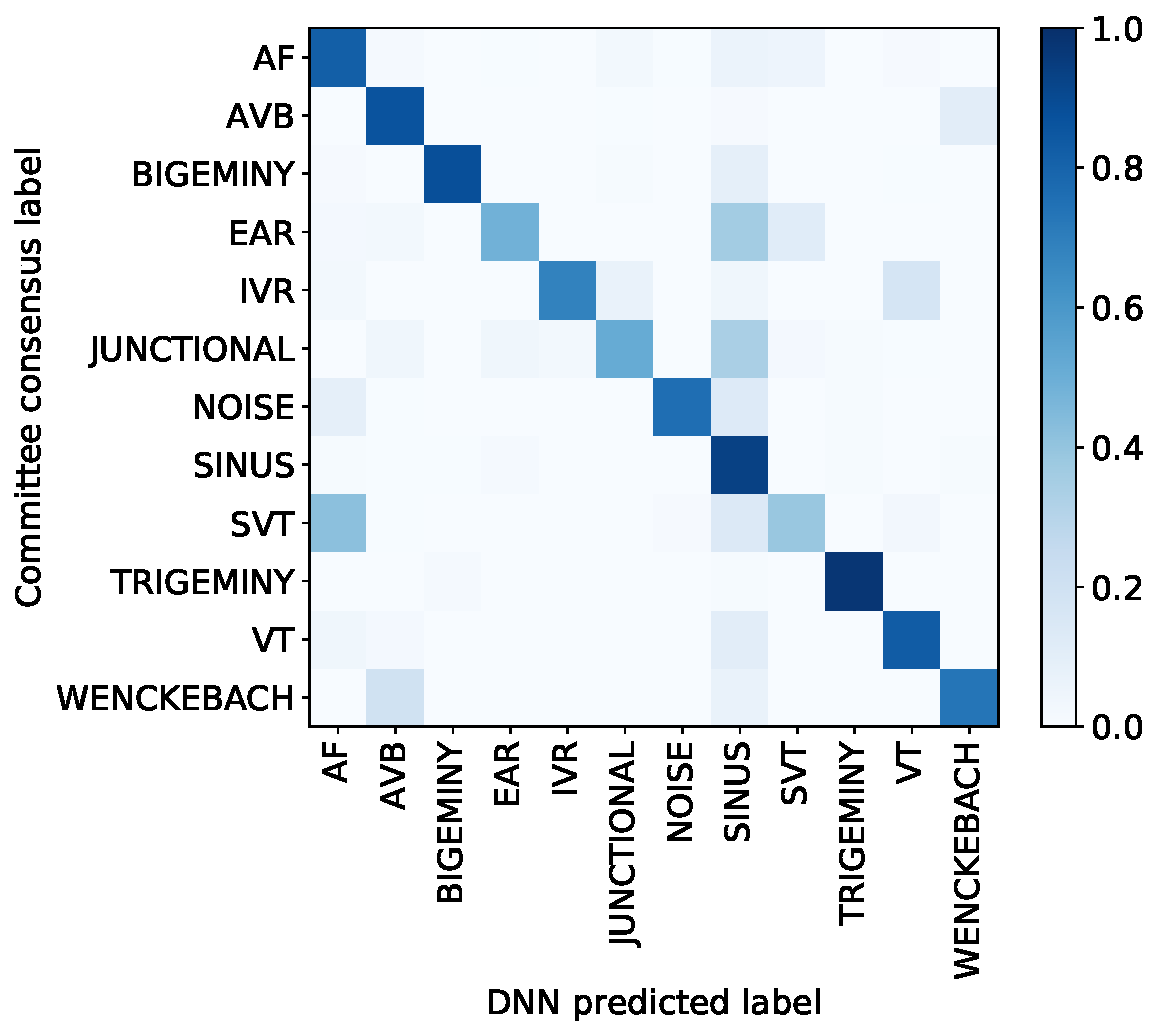
\includegraphics[width=0.9\linewidth]{arrhythmias/figures/model_confusions.pdf}
  \caption{Model}
  \label{fig:arrhythmia:model_confusion}
\end{subfigure}
\begin{subfigure}{.5\textwidth}
  \centering
  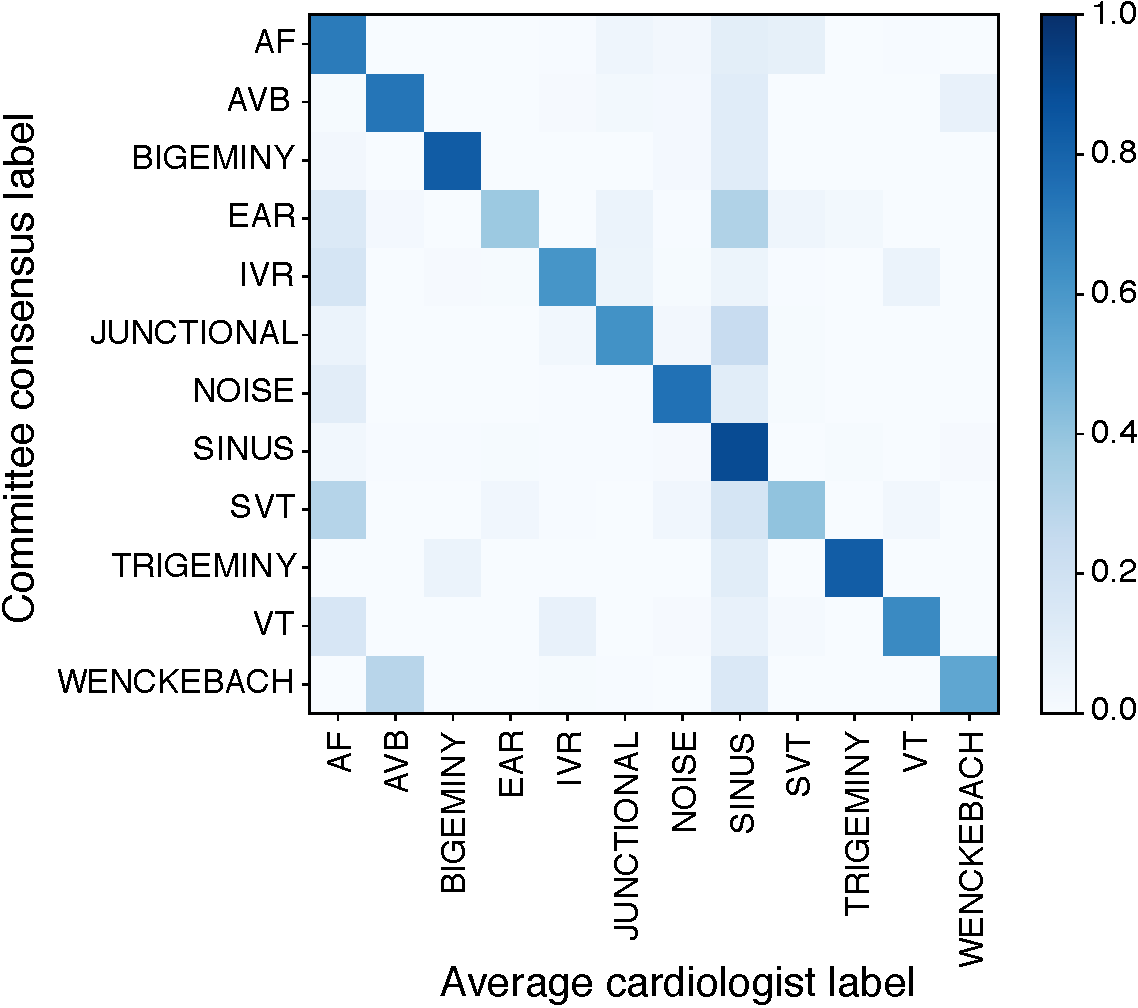
\includegraphics[width=0.9\linewidth]{arrhythmias/figures/human_confusions.pdf}
  \caption{Individual Cardiologists}
  \label{fig:arrhythmia:human_confusion}
\end{subfigure}
\caption{Confusion matrices for the model and individual cardiologist
         predictions with the committee consensus annotations as ground
         truth.}
\end{figure}

Often the mistakes made by the model are understandable. For example, confusing
Wenckebach and AVB\_Type2 makes sense given that the two rhythms in general
have very similar ECG morphologies. Similarly, Supraventricular Tachycardia
(SVT) and Atrial Fibrillation (AFIB) are often confused with Atrial Flutter
(AFL) which is understandable given that they are all atrial arrhythmias. We
also note that Idioventricular Rhythm (IVR) is sometimes mistaken as
Ventricular Tachycardia (VT), which again makes sense given that the two only
differ in heart-rate and are difficult to distinguish close to the 100 beats
per minute delineation.

One of the most common confusions is between Ectopic Atrial Rhythm (EAR) and
the sinus rhythm. The main distinguishing criteria for this rhythm is an
irregular P wave. This can be subtle to detect especially when the P wave has a
small amplitude or when noise is present in the signal.

\section{Conclusion}

We develop a model which exceeds the cardiologist performance in detecting a
wide range of heart arrhythmias from single-lead ECG records. Key to the
performance of the model is a large annotated dataset and a very deep
convolutional network which can map a sequence of ECG samples to a sequence of
arrhythmia annotations. 

On the clinical side, future work should investigate extending the set of
arrhythmias and other forms of heart disease which can be automatically
detected with high-accuracy from single or multiple lead ECG records. For
example we do not detect Ventricular Flutter or Fibrillation. We also do not
detect Left or Right Ventricular Hypertrophy, Myocardial Infarction or a number
of other heart diseases which do not necessarily exhibit as arrhythmias. Some
of these may be difficult or even impossible to detect on a single-lead ECG but
can often be seen on a multiple-lead ECG.

Given that more than 300 million ECGs are recorded annually, high-accuracy
diagnosis from ECG can save expert clinicians and cardiologists considerable
time and decrease the number of misdiagnoses. Furthermore, we hope that this
technology coupled with low-cost ECG devices enables more widespread use of the
ECG as a diagnostic tool in places where access to a cardiologist is difficult.


\chapter{First-pass Speech Recognition}

\section{Introduction}
\label{sec:first_pass:introduction}

Modern large vocabulary continuous speech recognition (LVCSR) systems are
complex and difficult to modify. Much of this complexity stems from the
paradigm of modeling words as sequences of sub-phonetic states with hidden
Markov models (HMMs). HMM-based systems require carefully-designed training
recipes to construct consecutively more complex HMM recognizers. The overall
difficulty of building, understanding, and modifying HMM-based LVCSR systems
has limited progress in speech recognition and isolated it from many advances
in related fields. 

Previous work demonstrated an HMM-free approach for training a speech
recognizer \cite{graves2014}. The authors use a neural network to directly
predict transcript characters given the audio of an utterance. This approach
discards many of the assumptions present in modern HMM-based LVCSR systems in
favor of treating speech recognition as a direct sequence transduction problem.
The approach trains a neural network using the connectionist temporal
classification (CTC) loss function, which amounts to maximizing the likelihood
of an output sequence by efficiently summing over all possible input-output
sequence alignments.  Using CTC the authors were able to train a neural network
to predict the character sequence of test utterances with a character error
rate (CER) under 10\% on the Wall Street Journal LVCSR corpus. While impressive
in its own right, these results are not yet competitive with existing HMM-based
systems in terms of word error rate (WER). Good word-level performance in
speech recognition often depends heavily upon a language model to provide a
prior probability over likely word sequences. 

To integrate language model information during decoding, the probabilities from
the CTC-trained neural network are used to rescore a lattice or n-best
hypothesis list generated by a state-of-the-art HMM-based system
\cite{graves2014}. This introduces a potentially confounding factor because an
n-best list constrains the set of possible transcriptions significantly.
Additionally, it results in an overall system which still relies on HMM speech
recognition infrastructure to achieve the final results. In contrast, we
present \emph{first-pass} decoding results which use a neural network and
language model to decode from scratch, rather than re-ranking an existing set
of hypotheses.

We describe a decoding algorithm which directly integrates a language model
with CTC-trained neural networks to search through the space of possible word
sequences. Our first-pass decoding algorithm enables CTC-trained models to
benefit from a language model without relying on an existing HMM-based system
to generate a word lattice. This removes the lingering dependence on
HMM-centric speech recognition toolkits and enables us to achieve fairly
competitive WER results with only a neural network and $n$-gram language model.

Deep neural networks (DNNs) are the most widely used neural network
architecture for speech recognition \cite{hinton2012}. DNNs are a fairly
generic architecture for classification and regression problems. In HMM-based
LVCSR systems, DNNs act as acoustic models by predicting the HMM's hidden state
given the acoustic input for a point in time. However, in such HMM-DNN systems
the temporal reasoning about an output sequence takes place within the HMM
rather than the neural network. CTC training of neural networks forces the
network to model output sequence dependencies rather than reasoning about
single time frames independently from others. To better handle such temporal
dependencies previous work with CTC used long short term memory (LSTM)
networks. LSTM is a neural network architecture was originally designed to
prevent the vanishing gradient problem of sigmoidal DNNs or temporally
recurrent deep neural networks (RDNNs) \cite{hochreiter1997}.

Our work uses RDNNs instead of LSTMs as a neural network architecture. RDNNs
are simpler overall, because there are only dense weight matrix connections
between subsequent layers. This simpler architecture is more amenable to
graphics processing unit (GPU) computing which can significantly reduce
training times. Recent work shows that with rectifier nonlinearities DNNs can
perform well in DNN-HMM systems without suffering from vanishing gradient
problems during optimization \cite{dahl2013, zeiler2013, maas2013}. This makes
us hopeful that RDNNs with rectifier nonlinearities may be able to perform
comparably to LSTMs which are specially engineered to avoid vanishing
gradients.

\section{Model}
\label{sec:first_pass:model}

We train neural networks using the CTC loss function to do maximum
likelihood training of letter sequences given acoustic features as
input. We consider a single utterance as a training example consisting
of an acoustic feature matrix $X$ and word transcription $Y$. The CTC
objective function maximizes the log probability $\log p(Y \mid X)$. We
reserve a full exposition of the loss function here because our
formulation follows exactly the previous work on using CTC to predict
the characters of an utterance transcription~\cite{graves2014, graves2006}. 

\subsection{Deep Neural Networks}
\label{sec:first_pass:model:dnn}

With the loss function fixed we must next define how we compute $p(c \mid
x_t)$, the predicted distribution over output characters $c$ given the audio
features $x_t$ at time $t$. While many function approximators are possible for
this task, we choose as our most basic model a DNN. A DNN computes the
distribution $p(c \mid x_t)$ using a series of hidden layers followed by an output
layer. Given an input vector $x_t$ the first hidden layer activations are a
vector computed as,
\begin{align*}
  h^{(1)} = \sigma(W^{(1)T} x_t + b^{(1)}).
\end{align*}
The matrix $W^{(1)}$ and vector $b^{(1)}$ are the weight matrix and bias vector
for the layer. The function $\sigma(\cdot)$ is a point-wise nonlinearity. We
use rectifier nonlinearities and thus choose, $\sigma(z) = \max (z, 0)$.

DNNs can have arbitrarily many hidden layers. After the first hidden
layer, the hidden activations $h^{(i)}$ for layer $i$ are computed as,
\begin{align*}
  h^{(i)} = \sigma(W^{(i)T} h^{(i-1)} + b^{(i)}).
\end{align*}

To obtain a proper distribution over the set of possible characters $c$ the
final layer of the network is a \emph{softmax} output layer of the form,
\begin{align*}
  p(c=c_k \mid x_t) = \frac{\exp(- ( W^{(s)T}_k h^{(i-1)} + b^{(s)}_k))}
  {\sum_j \exp(- ( W^{(s)T}_j h^{(i-1)} + b^{(s)}_j))},
\end{align*}
where $W^{(s)}_k$ is the $k$'th column of the output weight matrix $W^{(s)}$
and $b^{(s)}_k$ is a scalar bias term. 

We can compute a subgradient for all parameters of the DNN given a training
example and thus utilize gradient-based optimization techniques. Note that this
same DNN formulation is commonly used in DNN-HMM models to predict a
distribution over senones instead of characters.

\subsection{Recurrent Deep Neural Networks}

A transcription $W$ has many temporal dependencies which a DNN may not
sufficiently capture. At each timestep $t$ the DNN computes its output using
only the input features $x_t$, ignoring previous hidden representations and
output distributions. To enable better modeling of the temporal dependencies
present in a problem, we use a RDNN. In a RDNN we select one hidden layer $j$
to have a temporally recurrent weight matrix $W^{(f)}$ and compute the layer's
hidden activations as,
\begin{align*}
  h^{(j)}_t = \sigma(W^{(j)T} h^{(j-1)}_t +  W^{(f)T} h^{(j)}_{t-1} + b^{(j)}).
\end{align*}
Note that we now make the distinction $h^{(j)}_t$ for the hidden activation
vector of layer $j$ at timestep $t$ since it now depends upon the activation
vector of layer $j$ at time $t-1$.

When working with RDNNs, we found it important to use a modified version of the
rectifier nonlinearity. This modified function selects $\sigma(z) = \min( \max
(z, 0), 20)$ which clips large activations to prevent divergence during network
training. Setting the maximum allowed activation to 20 results in the clipped
rectifier acting as a normal rectifier function in all but the most extreme
cases.

Aside from these changes, computations for a RDNN are the same as those in a
DNN as described in \ref{sec:first_pass:model:dnn}. Like the DNN, we can
compute a subgradient for a RDNN using a method sometimes called
backpropagation through time. In our experiments we always compute the gradient
completely through time rather than truncating to obtain an approximate
subgradient.

\subsection{Bi-Directional Recurrent Deep Neural Networks}

While forward recurrent connections reflect the temporal nature of the audio
input, a perhaps more powerful sequence transduction model is a BRDNN, which
maintains state both forwards and backwards in time. Such a model can integrate
information from the entire temporal extent of the input features when making
each prediction. We extend the RDNN to form a BRDNN by again choosing a
temporally recurrent layer $j$. The BRDNN creates both a forward and backward
intermediate hidden representation which we call $h_t^{(f)}$ and $h_t^{(b)}$
respectively. 

We use the temporal weight matrices $W^{(f)}$ and $W^{(b)}$ to propagate
$h_t^{(f)}$ forward in time and $h_t^{(b)}$ backward in time respectively. We
update the forward and backward components via the equations,
\begin{align*}
    h^{(f)}_t &= \sigma(W^{(j)T} h^{(j-1)}_t +  W^{(f)T} h^{(f)}_{t-1} + b^{(j)}), \\
    h^{(b)}_t &= \sigma(W^{(j)T} h^{(j-1)}_t +  W^{(b)T} h^{(b)}_{t+1} + b^{(j)}).
\end{align*}

Note that the recurrent forward and backward hidden representations are
computed entirely independently from each other. As with the RDNN we use the
modified nonlinearity function $\sigma(z) = \min( \max (z,0), 20)$. To obtain
the final representation $h^{(j)}_t$ for the layer we sum the two temporally
recurrent components,
\begin{align}
\begin{split}
  h^{(j)}_t = h^{(f)}_t + h^{(b)}_t.
\end{split}
\end{align}

Aside from this change to the recurrent layer the BRDNN computes its output
using the same equations as the RDNN. As for other models, we can compute a
subgradient for the BRDNN directly to perform gradient-based optimization.

\section{Decoding}
\label{sec:first_pass:decoding}

%%% NOTATION KEY:
% \Sigma is extended alphabet including blank
% S and s_t is sequence and sequence item at time t including blank char
% T is time, 
% x_t is input at time t, X is full audio input of length T
% W is full word output
% \ell is character label prefix not including blanks
% p(c; x_t) is output of BDRNN at time t

Assuming an input of length $T$, the output of the neural network will be $p(c;
x_t)$ for $t = 1,\ldots,T$. Again, $p(c; x_t)$ is a distribution over possible
characters in the alphabet $\Sigma$, which includes the blank symbol, given
audio input $x_t$. In order to recover a character string from the output of
the neural network, as a first approximation, we take the \texttt{argmax} at
each time step. Let $S = (s_1,\ldots,s_T)$ be the character sequence where $s_t
= \argmax_{c \in \Sigma} p(c; x_t)$. The sequence $S$ is mapped to a
transcription by collapsing repeat characters and removing blanks. This gives a
sequence which can be scored against the reference transcription using both CER
and WER.

This first approximation lacks the ability to include the constraint of either
a lexicon or a language model. We propose a generic algorithm which is capable
of incorporating such constraints. Taking $X$ to be the acoustic input of time
$T$, we seek a transcription $W$ which maximizes the probability,
\begin{equation}
  \label{eq:joint} p_{\text{net}}(W ; X) p_{\text{lm}}(W).  
\end{equation} 
Here the overall probability of the transcription is modeled as the product of
two factors: $p_{\text{net}}$ given by the network and $p_{\text{lm}}$ given by
a language model prior. In practice the prior $p_{\text{lm}}(W)$, when given by
an $n$-gram language model, is too constraining and thus we down-weight it and
include a word insertion penalty (or bonus) as
\begin{equation}\label{eq:amlm}
    p_{\text{net}}(W ; X) p_{\text{lm}}(W)^\alpha |W|^\beta.
\end{equation}
Alogrithm \ref{alg:decode} attempts to find a word string $W$ which maximizes
equation \ref{eq:amlm}.
\begin{algorithm}[bt]
  \caption{Prefix Beam Search: The algorithm initializes the previous set of
prefixes $A_\text{prev}$ to the empty string. For each time step and every
prefix $\ell$ currently in $A_\text{prev}$, we propose adding a character from the
alphabet $\Sigma$ to the prefix. If the character is a blank, we do not extend
the prefix. If the character is a space, we incorporate the language model
constraint. Otherwise we extend the prefix and incorporate the output of the
network. All new active prefixes are added to $A_\text{next}$. We then set
$A_\text{prev}$ to include only the $k$ most probable prefixes of $A_\text{next}$.
The output is the $1$ most probable transcript, although the this can easily
be extended to return an $n$-best list.}\label{alg:decode}
  \begin{algorithmic}
    \State $p_b(\emptyset; x_{1:0}) \gets 1,\; p_{nb}(\emptyset; x_{1:0}) \gets 0$
    \State $A_{\text{prev}} \gets \{\emptyset\}$ 
    \For {$t = 1, \ldots, T$}
      \State $A_{\text{next}} \gets \{\}$
      \For {$\ell \; \text{\bf in} \; A_{\text{prev}}$}
	\For {$c \; \text{\bf in} \; \Sigma$}
	  \If {$c = \text{blank}$}
	    \State $p_b(\ell; x_{1:t}) \gets p(\text{blank}; x_t) 
		(p_b(\ell ; x_{1:t-1}) + p_{nb}(\ell ; x_{1:t-1}))$
	    \State $\mbox{add } \ell \mbox{ to } A_{\text{next}}$
	  \Else
	    \State $\ell^+ \gets \mbox{concatenate }\ell \mbox{ and } c$
	    \If {$c = \ell_\text{end}$}
	      \State $p_{nb}(\ell^+; x_{1:t}) \gets p(c; x_t)p_b(\ell ; x_{1:t-1})$
	      \State $p_{nb}(\ell; x_{1:t}) \gets p(c; x_t)p_b(\ell ; x_{1:t-1})$
	    \ElsIf {$c = \text{space}$}
	    \State $p_{nb}(\ell^+; x_{1:t}) \gets p(W(\ell^+)| W(\ell))^\alpha 
		p(c; x_t)(p_b(\ell ; x_{1:t-1}) + p_{nb}(\ell ; x_{1:t-1}))$
	    \Else
	      \State $p_{nb}(\ell^+; x_{1:t}) \gets p(c; x_t)
		(p_b(\ell; x_{1:t-1}) + p_{nb}(\ell; x_{1:t-1}))$
	    \EndIf
	    \If {$\ell^+ \; \text{\bf not in} \; A_\text{prev}$}
	      \State $p_{b}(\ell^+; x_{1:t}) \gets p(\text{blank}; x_t)
		(p_b(\ell^+; x_{1:t-1}) + p_{nb}(\ell^+; x_{1:t-1}))$
	      \State $p_{nb}(\ell^+; x_{1:t}) \gets p(c; x_t)p_{nb}(\ell^+; x_{1:t-1})$
	    \EndIf
	    \State $\mbox{add } \ell^+ \mbox{ to } A_{\text{next}}$
	  \EndIf
	\EndFor
      \EndFor
      \State $A_{\text{prev}} \gets k 
	\text{ most probable prefixes in } A_{\text{next}}$
    \EndFor
    \State \Return $1 \text{ most probable prefix in } A_{\text{prev}}$
  \end{algorithmic}
\end{algorithm}
The algorithm maintains two separate probabilities for each prefix,
$p_{b}(\ell; x_{1:t})$ and $p_{nb}(\ell; x_{1:t})$. Respectively, these are the
probability of the prefix $\ell$ ending in blank or not ending in blank given
the first $t$ time steps of the audio input $X$.

The sets $A_{\text{prev}}$ and $A_{\text{next}}$ maintain a list of active
prefixes at the previous time step and proposed prefixes at the next time step
respectively. Note that the size of $A_{\text{prev}}$ is never larger than the
beam width $k$. The overall probability of a prefix is the product of a word
insertion term and the sum of the blank and non-blank ending probabilities,
\begin{equation}\label{eq:prefixprob}
  p(\ell; x_{1:t}) = (p_b(\ell; x_{1:t}) + p_{nb}(\ell; x_{1:t})) |W(\ell)|^\beta,
\end{equation}
where $W(\ell)$ is the set of words in the sequence $\ell$. When taking the $k$
most probable prefixes of $A_{\text{next}}$, we sort each prefix using the
probability given by equation \ref{eq:prefixprob}.

The variable $\ell_{\text{end}}$ is the last character in the label sequence
$\ell$. The function $W(\cdot)$, which converts $\ell$ into a string of words,
segments the sequence $\ell$ at each space character and truncates any
characters trailing the last space. 

We incorporate a lexicon or language model constraint by including the
probability $p(W(\ell^+) | W(\ell))$ whenever the algorithm proposes appending
a space character to $\ell$. By setting $p(W(\ell^+) | W(\ell))$ to $1$ if the
last word of $W(\ell^+)$ is in the lexicon and $0$ otherwise, the probability
acts as a constraint forcing all character strings $\ell$ to consist of only
words in the lexicon.  Furthermore, $p(W(\ell^+) | W(\ell))$ can represent a
$n$-gram language model by considering only the last $n-1$ words in $W(\ell)$.  


\section{Experiments}

We evaluate our approach on the 81 hour Wall Street Journal (WSJ) news article
dictation corpus (available in the LDC catalog as LDC94S13B and LDC93S6B). Our
training set consists of 81 hours of speech from 37,318 utterances. The basic
preparation of transforming the LDC-released corpora into training and test
subsets follows the Kaldi speech recognition toolkit's s5
recipe~\cite{povey2011}. However, we did not apply much of the text
normalization used to prepare transcripts for training an HMM system. Instead
we simply drop unnecessary transcript notes like lexical stress, keeping
transcribed word fragments and acronym punctuation marks. We can safely discard
much of this normalization because our approach does not rely on a lexicon or
pronunciation dictionary, which cause problems especially for word fragments.
Our language models are the standard models released with the WSJ corpus
without lexical expansion. We used the `dev93' evaluation subset as a
development set and report final test set performance on the `eval92'
evaluation subset. Both subsets use the same 20k word vocabulary. The language
model used for decoding is constrained to this same 20k word vocabulary.

The input audio was converted into log-Mel filterbank features with 23
frequency bins. A context window of +/- 10 frames were concatenated to form a
final input vector of size 483. We did not perform additional feature
preprocessing or feature-space speaker adaptation.  Our output alphabet
consists of 32 classes, namely the blank symbol ``\_'', 26 letters, 3
punctuation marks (apostrophe, ., and -) as well as tokens for noise and space. 

\subsection{First-Pass Decoding with a Language Model}

We trained a BRDNN with 5 hidden layers, all with 1824 hidden units, for a
total of 20.9M free parameters. The third hidden layer of the network has
recurrent connections. Weights in the network are initialized from a uniform
random distribution scaled by the weight matrix's input and output layer
size~\cite{glorot2011}. We use the Nesterov accelerated gradient optimization
algorithm~\cite{sutskever2013} with initial learning rate $10^{-5}$, and
maximum momentum 0.95. After each full pass through the training set we divide
the learning rate by 1.2 to ensure the overall learning rate decreases over
time. We train the network for a total of 20 passes over the training set,
which takes about 96 hours using our Python GPU implementation.  For decoding
with prefix search we use a beam size of 200 and cross-validate with a held-out
set to find a good setting of the parameters $\alpha$ and $\beta$.
Table~\ref{tab:first_pass:res_decode} shows word and character error rates for
multiple approaches to decoding with this trained BRDNN.

\begin{table}
\centering
\begin{tabular}{lrr}
\toprule
Model & CER & WER\\
\midrule
No LM         & 10.0 & 35.8 \\
Dictionary LM & 8.5  & 24.4 \\
Bigram LM     & 5.7  & 14.1 \\
\bottomrule
\end{tabular}
\caption{Word error rate (WER) and character error rate (CER) results
  for a BDRNN trained with the CTC loss function.}
\label{tab:first_pass:res_decode}
\end{table}

Without any sort of language constraint WER is quite high, despite the fairly
low CER. This is consistent with our observation that many mistakes at the
character level occur when a word appears mostly correct but does not conform
to the highly irregular orthography of English. Prefix-search decoding using
the 20k word vocabulary as a prior over possible character sequences results in
a substantial WER improvement, but changes the CER relatively little. Comparing
the CERs of the no LM and dictionary LM approaches again demonstrates that
without an LM the characters are mostly correct but are distributed across many
words which increases WER. A large relative drop in both CER and WER occur when
we decode with a bigram LM. Performance of the bigram LM model demonstrates
that CTC-trained systems can attain competitive error rates without relying on
a lattice or n-best list generated by an existing speech system.

\subsection{The Effect of Recurrent Connections}

Previous experiments with DNN-HMM systems found minimal benefits from recurrent
connections in DNN acoustic models. It is natural to wonder whether recurrence,
and especially bi-directional recurrence, is an essential aspect of our
architecture. To evaluate the impact of recurrent connections we compare the
train and test CERs of DNN, RDNN, and BRDNN models while roughly controlling
for the total number of free parameters in the model.
Table~\ref{tab:first_pass:res_recurrence} shows the results for each type of
architecture. 

\begin{table}
\centering
\begin{tabular}{lrrr}
\toprule
Model & Parameters (M) & Train CER & Test CER \\
\midrule
DNN   & 16.8 & 3.8 & 22.3 \\
RDNN  & 22.0 & 4.2 & 13.5 \\
BRDNN & 20.9 & 2.8 & 10.7 \\
\bottomrule
\end{tabular}
\caption{Train and test set CER results for a DNN without recurrence, an RDNN,
         and a BRDNN.}
\label{tab:first_pass:res_recurrence}
\end{table}

Both variants of recurrent models show substantial test set CER improvements
over the non-recurrent DNN model. Note that we report performance for a DNN of
only 16.8M total parameters which is smaller than the total number of
parameters used in both the RDNN and BRDNN models. We found that larger DNNs
performed worse on the test set, suggesting that DNNs may be more prone to
over-fitting for this task. Although the BRDNN has fewer parameters than the
RDNN it performs better on both the training and test sets. Again this suggests
that the architecture itself drives improved performance rather than the total
number of free parameters. Conversely, because the gap between bi-directional
recurrence and single recurrence is small relative to a non-recurrent DNN,
on-line speech recognition using a singly recurrent network may be feasible
without overly damaging performance.

\section{Conclusion}

We presented a decoding algorithm which enables first-pass LVCSR with a
language model for CTC-trained neural networks. This decoding approach removes
the lingering dependence on HMM-based systems found in previous work.
Furthermore, first-pass decoding demonstrates the capabilities of a CTC-trained
system without the confounding factor of potential effects from pruning the
search space via a provided lattice. While our results do not outperform the
best HMM-based systems on the WSJ corpus, they demonstrate the promise of
CTC-based speech recognition systems.

Our experiments with the BRNN further simplify the infrastructure needed to
create CTC-based speech recognition systems. The BRNN is overall a less complex
architecture than LSTMs and can relatively easily be made to run on GPUs since
large matrix multiplications dominate the computation. However, our experiments
suggest that recurrent connections are critical for good performance.
Bi-directional recurrence helps beyond unidirectional recurrence but could be
sacrificed in cases that require low-latency, online speech recognition. Taken
together with previous work on CTC-based LVCSR, we believe there is an exciting
path forward for high quality LVCSR without the complexity of HMM-based
infrastructure.


\chapter{Conclusions}

This is the conclusion.


%\appendix
%\include{appendix1}

\bibliographystyle{plain}
\bibliography{refs}

\end{document}

